When allowing on/off photodetectors, an intuitive approach to the discrimination of binary coherent states can be constructed~\cite{Kennedy1973a}. Assuming we know the amplitude $|\alpha|$ of the incoming states, we can readily displace the signal by $\weyl{\beta}$ with $\beta = \alpha$. In this way, if $\ket{-\alpha}$ was received, the resulting state would be $\ket{0}$, and if $\ket{\alpha}$ was received instead, the resulting state would be $\ket{2\alpha}$. This is illustrated in Fig.~\ref{fig:312shifts}, where the Wigner function of the incoming states (either $\ket{\alpha}$ or $\ket{-\alpha}$, with equal priors)
is shown, along with the displaced signals.
 \begin{figure}[t!]
 \centering
     \begin{subfigure}[b]{0.49\textwidth}
         \centering
         \includegraphics[width=1.\textwidth]{Figures/some_wigners/bpshcoh.png}
         \caption{}
         \label{fig:312shiftsA}
     \end{subfigure}
     \hfill
     \begin{subfigure}[b]{0.49\textwidth}
         \centering
         \includegraphics[width=1.\textwidth]{Figures/some_wigners/bpshcohdisp.png}
         \caption{}
         \label{fig:312shiftsB}
     \end{subfigure}
 \caption{We show the Wigner functions for (panel $a$) the coherent states $\ket{\pm \alpha}$ and (panel $b$) the displaced coherent states $\ket{0}$ and $\ket{2 \alpha}$}
 \label{fig:312shifts}
 \end{figure}
After displacing, an on/off photodetector is used, which projects the probe into the vacuum state $\ket{0}$ or its complement, \textit{i.e.} $\mathcal{M}_{ph} = \llaves{\proj{0}, \mathbb{I}-\proj{0}}$. Such a measurement is a non-Gaussian one, yet is a standard component in modern quantum optics laboratories. The whole apparatus of measuring the displaced signal is known as the \textit{Kenendy receiver}, and is shown in Fig.~\ref{fig:kennedy_receiver}.

Thus, once the measurement outcome is obtained, a guess for the most-likely hypothesis needs to be performed. By denoting the measurement outcome by $o\in\llaves{0,1}$ (standing for zero and one or more photons detected respectively), the sucess probability reads
\begin{align}
P^{ken}_s = \sum_{o=0,1} \underset{k}{\text{max }} p_k p(o|\alpha^{(k)}),
\end{align}
where $p(n|\alpha^{(k)})$ can easily be obtained by noticing that $p(0|\alpha^{(k)}) = |\langle 0 | \hat{D}_\beta \ket{\alpha}|^2 = |\langle -\beta | \alpha \rangle|^2$, and $p(1|\alpha^{(k)}) = 1- p(0|\alpha^{(k)})$.
\begin{figure}[b!]
    \centering
    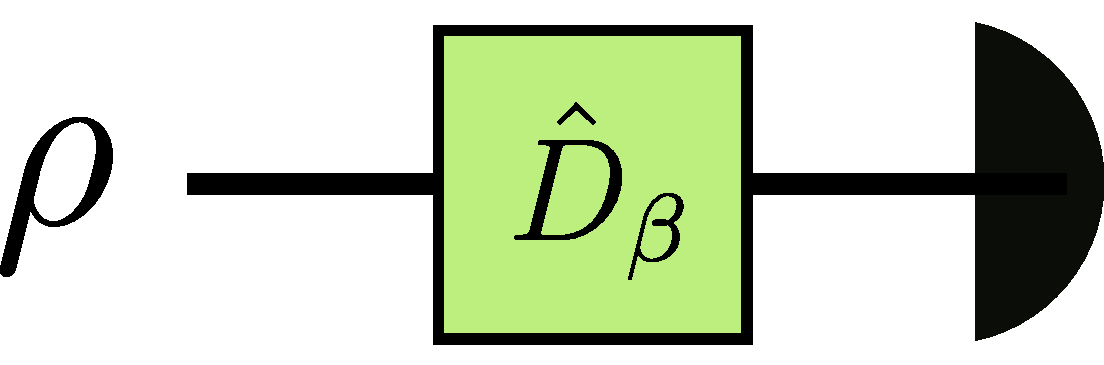
\includegraphics[width=0.5\textwidth]{Figures/312/kennedy_receiver.pdf}
    \caption{We show the Kennedy receiver, which in the case of coherent states' intensity being $\alpha$, it reduces to $\beta = -\alpha$.}
    \label{fig:kennedy_receiver}
\end{figure}

Let us understand the logic behind this receiver. Once displaced, the signal can either be $\ket{0}$ or $\ket{2\alpha}$. In the former case, when measuring with an on/off photodetection --- and in the absense of errors such as dark-counts --- the only possible result is $n=0$ photons. Thus, if outcome $n=1$ was obtained, we can be sure that the signal is $\ket{\alpha}$. However, outcome $n=0$ does not imply that the signal is $\ket{-\alpha}$ with absolute certainty, since $|\braket{0}{2\alpha}|^2 = e^{-4|\alpha^2|}\neq0$. This leads us to evaluate the success probability of Kennedy receiver as:
\begin{align}\label{eq:ps_ken}
P_s^{\text{ken}}(\alpha) = 1 - \frac{e^{-4|\alpha|^2}}{2}.
\end{align}
When compared with the homodyne measurement (\textit{i.e.} Eq.~\ref{eq:gaussian_receiver_homo}), we observe that an advantage in favour of Kennedy receiver is only attained when $|\alpha| \gtrsim 0.4$.

As it happens in cases where little resources are available, each component of a protocol should be optimized if possible. Here, we can readily observe that the displacement value $\beta=\alpha$ might not be the best choice.

\subsubsection{Optimized Kennedy receiver}
By identifying the displacement as a degree of freedom to be optimized, we have $\textit{parametrized}$ the Kennedy receiver, and its performance is now measured by the success probability associated to the specific choice of $\beta$. For a fixed $\beta$, we will denote such receiver as the $\beta$-Kennedy receiver (the original Kennedy receiver is recovered for $\beta = \alpha$).

We note that different values of $\beta$ will lead to different POVMs $\mathcal{M}_\beta$, each belonging to the same family of Kennedy-like receivers. This is analogous to the case of parametrized quantum circuits studied in Sec.~\ref{sec:1_nisq}, in which a unitary transformation was constructed from local qubit rotations and entangling CNOT gates, and optimized in such a way to minimize a given cost function. From this quantum machine learning point of view, the parametrized quantum circuit analogous is given by $\mathcal{M}_\beta$ and the success probability (or, equivalently, the error probability) $P^{\beta-\text{ken}}_e(\alpha, \beta)$ plays the role of the cost function.

Depending on the context, this problem also falls into the category of \textit{optimal control theory}~\cite{Bell1964, Bert05}, since one is interested in optimizing the cost function. This field tries to find answers on how to steer a system towards a target state by performing external controls or \textit{actions} on it. For instance, such system can be thought as our coherent state $\ket{\alpha^{(k)}}$, whose phase needs to be deciphered by the $\beta$-Kennedy receiver, and different actions correspond to varying the value of $\beta$. In this regard, navigating through the optimization landscape is important in order to find which actions are the best, though doing so is generally hard. For instance, one needs to estimate the cost value for each possible value of the control: in our discrimination example, this means estimating the success probability associated to each possible $\beta$-Kennedy receiver out of several repetitions of the discrimination experiment. While estimating the entire landscape is generally too costly, we can get some insight into the problem at hand by studying simplified models. In particular, certain scenarios can readily be deemed \textit{hopeless}, in the sense that parameter optimization might only succeed with an exponentially vanishing success probability, as it happens with barren plateaus appearing in certain parametrized quantum circuits (see  Sec.~\ref{sec:1_nisq})

\begin{figure}[t!]
    \centering
    \includegraphics[width=.9\textwidth]{Figures/kenn_landscape.pdf}
    \caption{We show the optimization landscape for the $\beta$-Kennedy receiver, at a fixed intensity $\alpha=0.2$. which in the case of coherent states' intensity being $\alpha$, it reduces to $\beta = -\alpha$.}
    \label{fig:optiland}
\end{figure}

In this chapter, the simplified model that allows us to get some insight is precisely the $\beta$-Kennedy receiver, whose optimization landscape is shown in Fig.~\ref{fig:optiland} for a fixed value of $\alpha=0.2$. In this a region, the homodyne receiver outperforms the Kennedy one, as noticed after inspecting Eq.~\ref{eq:ps_ken}. However, we observe that there is an entire region of $\beta$ values for which the $\beta$-Kennedy receiver can actually surpass the homodyne limit. Note also that the optimal solution is degenerate; this is a consequence of the symmetry in testing either $\ket{\alpha}$ (negative $\beta$) or $\ket{-\alpha}$ (positive $\beta$) using the photon-detector logic explained above.

\begin{figure}[t!]
\centering
    \begin{subfigure}[b]{0.49\textwidth}
        \centering
        \includegraphics[width=1.\textwidth]{Figures/312/kennedy_compa.pdf}
    \end{subfigure}
    \hfill
    \begin{subfigure}[b]{0.49\textwidth}
        \centering
        \includegraphics[width=1.\textwidth]{Figures/312/kennedy_compa_diff_hel.pdf}
    \end{subfigure}
\caption{We compare the success probabilities for homodyne receiver, Kennedy receiver, and optimized-Kennedy receiver with the Helstrom bound. Data in both panels is the same, however in right one we show the different with Helstrom bound, in order to help visualization.}
\label{fig:kenn_compa1}
\end{figure}

In this way, the optimization over $\beta$ can be carried out for each value of $\alpha$. The resulting receiver is known as the \textit{optimized Kennedy receiver}, and surpasses the homodyne limit for all intensity values, as shown in Fig.~\ref{fig:kenn_compa1}, where we compare its success probability, denoted by $P_S^{opt-\text{ken}}$, with that of homodying and with the original Kennedy receiver $P_S^{\text{ken}}$ (\textit{e.g.} $\beta = -\alpha$). To aid the comparison, we have depicted the difference with respect to the Helstrom bound: how to approach such a limit is the matter of the next section.

%
